% Framed knot as ribbon — unknot K with push-off K_f, one twist (Ch 5/6)
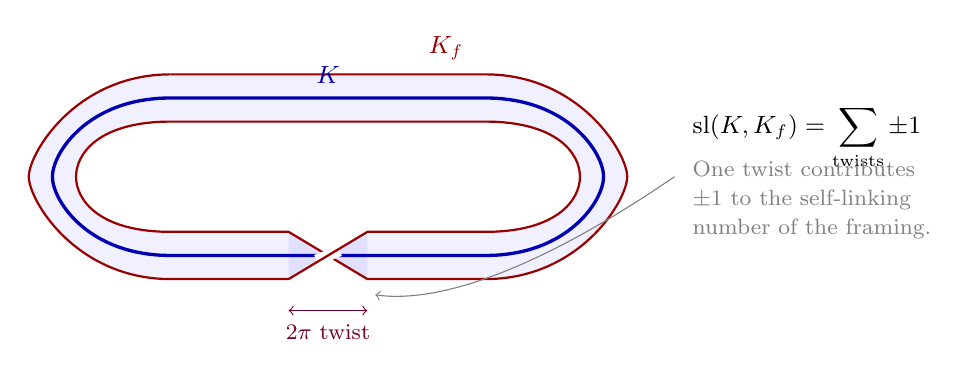
\begin{tikzpicture}[thick,
    knot/.style={very thick, blue!70!black},
    pushoff/.style={thick, red!60!black},
    annotation/.style={thin, purple!60!black}]

  % === Unknot K thickened into a ribbon with one full twist ===
  %
  % Layout: elongated oval (racetrack shape) oriented horizontally.
  %   - K is the core curve (center of the ribbon).
  %   - K_f is the push-off (upper edge everywhere except through
  %     the twist, where it crosses to the lower edge and back).
  %   - One twist is placed in the bottom-center segment.

  % Coordinates:
  %   Top segment:   y = 2.0 (K at 2.0, edges at 1.7 and 2.3)
  %   Bottom segment: y = 0.0 (K at 0.0, edges at -0.3 and 0.3)
  %   Left arc center:  x = 0.5
  %   Right arc center: x = 6.5
  %   Twist center: x = 3.5 (bottom segment)

  \def\w{0.3}  % half-width of ribbon

  % --- Ribbon shading ---
  % Top band
  \fill[blue!6] (1.5, 2.0-\w) rectangle (5.5, 2.0+\w);
  % Bottom band (left of twist)
  \fill[blue!6] (1.5, 0.0-\w) rectangle (3.0, 0.0+\w);
  % Bottom band (right of twist)
  \fill[blue!6] (4.0, 0.0-\w) rectangle (5.5, 0.0+\w);
  % Left semicircle band
  \fill[blue!6]
    (1.5, 2.0+\w) .. controls (0.3, 2.0+\w) and (-0.3, 1.3)
      .. (-0.3, 1.0)
    .. controls (-0.3, 0.7) and (0.3, 0.0-\w) .. (1.5, 0.0-\w)
    -- (1.5, 0.0+\w)
    .. controls (0.6, 0.0+\w) and (0.3, 0.7) .. (0.3, 1.0)
    .. controls (0.3, 1.3) and (0.6, 2.0-\w) .. (1.5, 2.0-\w)
    -- cycle;
  % Right semicircle band
  \fill[blue!6]
    (5.5, 2.0+\w) .. controls (6.7, 2.0+\w) and (7.3, 1.3)
      .. (7.3, 1.0)
    .. controls (7.3, 0.7) and (6.7, 0.0-\w) .. (5.5, 0.0-\w)
    -- (5.5, 0.0+\w)
    .. controls (6.4, 0.0+\w) and (6.7, 0.7) .. (6.7, 1.0)
    .. controls (6.7, 1.3) and (6.4, 2.0-\w) .. (5.5, 2.0-\w)
    -- cycle;

  % Twist region (cross-hatched look via darker fill)
  \fill[blue!18, opacity=0.65]
    (3.0, \w) -- (4.0, -\w) -- (4.0, \w) -- (3.0, -\w) -- cycle;

  % --- Central curve K ---
  \draw[knot]
    (1.5, 2.0)  -- (5.5, 2.0)             % top
    .. controls (6.55, 2.0) and (7.0, 1.3) .. (7.0, 1.0)   % right arc
    .. controls (7.0, 0.7) and (6.55, 0.0) .. (5.5, 0.0)   % right arc
    -- (4.0, 0.0) -- (3.0, 0.0) -- (1.5, 0.0)              % bottom
    .. controls (0.45, 0.0) and (0.0, 0.7) .. (0.0, 1.0)   % left arc
    .. controls (0.0, 1.3) and (0.45, 2.0) .. (1.5, 2.0);  % left arc

  % --- Push-off K_f ---
  % Follows upper edge (+w) everywhere except through the twist region,
  % where it crosses from +w to -w (creating a crossing with the other edge).

  % Top and right arc (upper edge)
  \draw[pushoff]
    (1.5, 2.0+\w) -- (5.5, 2.0+\w)
    .. controls (6.7, 2.0+\w) and (7.3, 1.3) .. (7.3, 1.0)
    .. controls (7.3, 0.7) and (6.7, 0.0-\w) .. (5.5, 0.0-\w)
    -- (4.0, 0.0-\w);

  % Twist: K_f crosses from lower edge (-w) to upper edge (+w)
  % Over-strand (drawn on top)
  \draw[pushoff, line cap=round] (4.0, -\w) -- (3.0, \w);

  % Left segment and arc (upper edge, after crossing)
  \draw[pushoff]
    (3.0, 0.0+\w) -- (1.5, 0.0+\w)
    .. controls (0.6, 0.0+\w) and (0.3, 0.7) .. (0.3, 1.0)
    .. controls (0.3, 1.3) and (0.6, 2.0-\w) .. (1.5, 2.0-\w)
    -- (5.5, 2.0-\w)
    .. controls (6.4, 2.0-\w) and (6.7, 1.3) .. (6.7, 1.0)
    .. controls (6.7, 0.7) and (6.4, 0.0+\w) .. (5.5, 0.0+\w)
    -- (4.0, 0.0+\w);

  % Under-strand of twist (other edge going from +w to -w)
  % White gap for crossing visibility
  \draw[white, line width=4pt] (3.35, -0.06) -- (3.65, 0.06);
  \draw[pushoff, line cap=round] (4.0, \w) -- (3.0, -\w);

  % Continue the lower edge after twist
  \draw[pushoff]
    (3.0, 0.0-\w) -- (1.5, 0.0-\w)
    .. controls (0.3, 0.0-\w) and (-0.3, 0.7) .. (-0.3, 1.0)
    .. controls (-0.3, 1.3) and (0.3, 2.0+\w) .. (1.5, 2.0+\w);

  % === Labels ===
  \node[knot, above, font=\small] at (3.5, 2.05) {$K$};
  \node[red!60!black, above, font=\small] at (5.0, 2.35) {$K_f$};

  % Twist annotation
  \draw[annotation, <->] (3.0, -0.7) -- (4.0, -0.7);
  \node[below, font=\footnotesize, purple!60!black] at (3.5, -0.75)
    {$2\pi$ twist};

  % Self-linking formula
  \node[right, font=\small, align=left] at (8.0, 1.5)
    {$\mathrm{sl}(K, K_f) = \displaystyle\sum_{\mathrm{twists}} \pm 1$};
  \node[right, font=\footnotesize, gray, align=left] at (8.0, 0.7)
    {One twist contributes\\[1pt]
     $\pm 1$ to the self-linking\\[1pt]
     number of the framing.};

  % Arrow to twist region
  \draw[->, thin, gray] (7.9, 1.0)
    .. controls (6.0, -0.3) and (4.8, -0.6) .. (4.1, -0.5);

\end{tikzpicture}
